\documentclass{../paper}

\begin{document}

\title{X-ray Diffraction \\ {\em Post-lab}}

\author{Iago B.~Mendes\,\orcidlink{0009-0007-9845-8448}}
\email{ibrazmen@oberlin.edu}
\affiliation{Department of Physics and Astronomy, Oberlin College, Oberlin, Ohio 44074, USA}

\date{\today}

\maketitle

\section{Background}

In this experiment, we use x-ray diffraction to analyze the crystal structure of many samples.

\begin{figure}
  \centering
  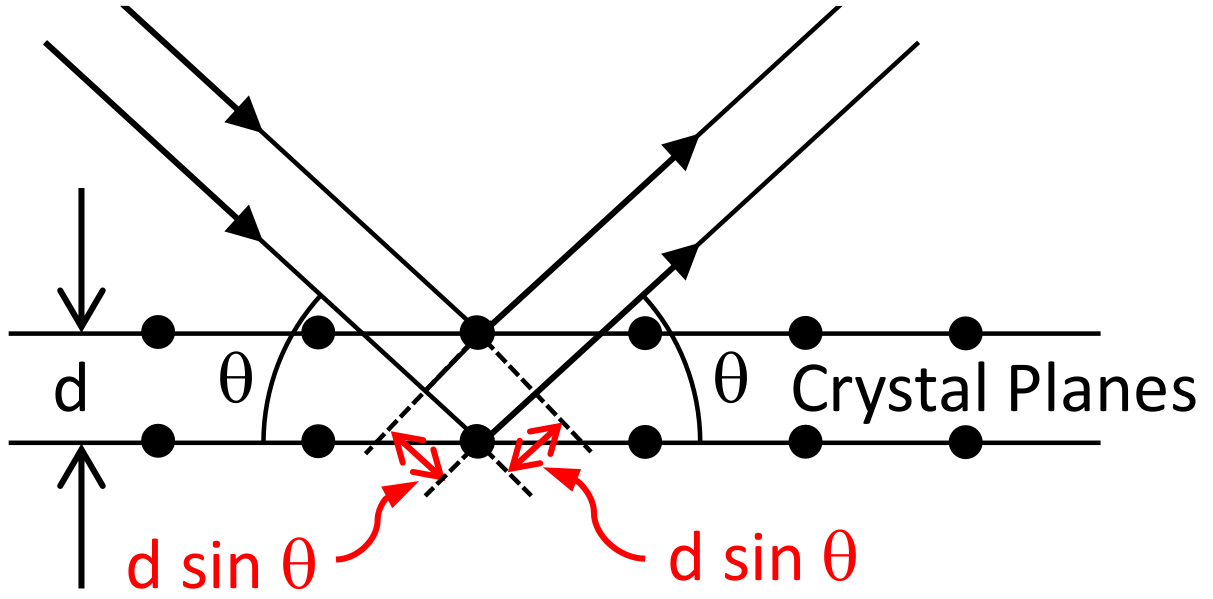
\includegraphics[width=0.6\columnwidth]{assets/bragg-scattering.png}
  \caption{Schematic representation of Bragg scattering. This figure is reproduced from \cite{LabManual}}
  \label{fig:angles}
\end{figure}

\section{Procedure}


\section{Results}


\begin{acknowledgements}
  This work was done in collaboration with Sage Weisrock under the supervision of Professor Yumi Ijiri.
\end{acknowledgements}

\bibliography{refs}

\end{document}
